%%%%%%%%%%%%%%%%%%%%%%%%%%%%%%%%%%%%%%%%%
% Beamer Presentation
% LaTeX Template
% Version 1.0 (10/11/12)
%
% This template has been downloaded from:
% http://www.LaTeXTemplates.com
%
% License:
% CC BY-NC-SA 3.0 (http://creativecommons.org/licenses/by-nc-sa/3.0/)
%
%%%%%%%%%%%%%%%%%%%%%%%%%%%%%%%%%%%%%%%%%

%----------------------------------------------------------------------------------------
%	PACKAGES AND THEMES
%----------------------------------------------------------------------------------------

\documentclass{beamer}

\mode<presentation> {

% The Beamer class comes with a number of default slide themes
% which change the colors and layouts of slides. Below this is a list
% of all the themes, uncomment each in turn to see what they look like.

%\usetheme{default}
%\usetheme{AnnArbor}
%\usetheme{Antibes}
%\usetheme{Bergen}
%\usetheme{Berkeley}
\usetheme{Berlin}
%\usetheme{Boadilla}
%\usetheme{CambridgeUS}
%\usetheme{Copenhagen}
%\usetheme{Darmstadt}
%\usetheme{Dresden}
%\usetheme{Frankfurt}
%\usetheme{Goettingen}
%\usetheme{Hannover}
%\usetheme{Ilmenau}
%\usetheme{JuanLesPins}
%\usetheme{Luebeck}
%\usetheme{Madrid}
%\usetheme{Malmoe}
%\usetheme{Marburg}
%\usetheme{Montpellier}
%\usetheme{PaloAlto}
%\usetheme{Pittsburgh}
%\usetheme{Rochester}
%\usetheme{Singapore}
%\usetheme{Szeged}
%\usetheme{Warsaw}

% As well as themes, the Beamer class has a number of color themes
% for any slide theme. Uncomment each of these in turn to see how it
% changes the colors of your current slide theme.

%\usecolortheme{albatross}
%\usecolortheme{beaver}
%\usecolortheme{beetle}
%\usecolortheme{crane}
%\usecolortheme{dolphin}
%\usecolortheme{dove}
%\usecolortheme{fly}
%\usecolortheme{lily}
%\usecolortheme{orchid}
%\usecolortheme{rose}
%\usecolortheme{seagull}
%\usecolortheme{seahorse}
%\usecolortheme{whale}
%\usecolortheme{wolverine}

%\setbeamertemplate{footline} % To remove the footer line in all slides uncomment this line
%\setbeamertemplate{footline}[page number] % To replace the footer line in all slides with a simple slide count uncomment this line
\setbeamertemplate{headline}{}
\setbeamertemplate{navigation symbols}{} % To remove the navigation symbols from the bottom of all slides uncomment this line
}

  \setbeamertemplate{footline}%{miniframes theme}
  {%
    \begin{beamercolorbox}[colsep=1.5pt]{upper separation line foot}
    \end{beamercolorbox}
    \begin{beamercolorbox}[ht=2.5ex,dp=1.125ex,%
      leftskip=.3cm,rightskip=.3cm plus1fil]{author in head/foot}%
      \leavevmode{\usebeamerfont{author in head/foot}\insertshortauthor}%
      \hfill%
      {\usebeamerfont{institute in head/foot}\usebeamercolor[fg]{institute in head/foot}\insertshortinstitute}%
    \end{beamercolorbox}%
    \begin{beamercolorbox}[ht=2.5ex,dp=1.125ex,%
      leftskip=.3cm,rightskip=.3cm plus1fil]{title in head/foot}%
      {\usebeamerfont{title in head/foot}\insertshorttitle} \hfill     \insertframenumber/\inserttotalframenumber%
    \end{beamercolorbox}%
    \begin{beamercolorbox}[colsep=1.5pt]{lower separation line foot}
    \end{beamercolorbox}
  }



\usepackage{graphicx} % Allows including images
\usepackage{booktabs} % Allows the use of \toprule, \midrule and \bottomrule in tables
\usepackage[utf8]{inputenc}
\usepackage[magyar]{babel}
\usepackage{fixltx2e}
\usepackage{epstopdf}
\usepackage{xcolor}
\usepackage{pdfpages}
\usepackage{listings}



%----------------------------------------------------------------------------------------
%	TITLE PAGE
%----------------------------------------------------------------------------------------

\title[Big Data elemzési eszközök nyílt forráskódú platformokon]{Big Data elemzési eszközök nyílt forráskódú platformokon\\ Házi feladat} % The short title appears at the bottom of every slide, the full title is only on the title page

\author{Mátyás-Barta Csongor} % Your name

\institute[BME] % Your institution as it will appear on the bottom of every slide, may be shorthand to save space
{
VYW0YR\\
mbcsongor@yahoo.com \\% Your email address
}
\date{\today} % Date, can be changed to a custom date

\begin{document}


\begin{frame}[plain]
\titlepage % Print the title page as the first slide
\end{frame}

\begin{frame}
\frametitle{Választott feladatok és technológiák} 	
	\begin{itemize}
		\item Flight1 - Melyik reptéren gurulnak (TaxiIn és TaxiOut) átlagosan legtöbbet a gépek? 
			\begin{center}
				
\includegraphics[height=1cm]{figures/mapreduce}
			\end{center}			
		\item Flight4 - Melyik 10 légitársaság indul a legtöbbször későn (DepDelay)?
			\begin{center}
				
\includegraphics[height=1cm]{figures/spark}
			\end{center}	
		\item Flight2 - Honnan szállt fel a legtöbb repülő? 
			\begin{center}
				
\includegraphics[height=2cm]{figures/pig}
			\end{center}	
	\end{itemize}
\end{frame}
%----------------------------------------------------------------------------------------
%	PRESENTATION SLIDES
%----------------------------------------------------------------------------------------

%------------------------------------------------
\section{Flight1 - Java MapReduce} % Sections can be created in order to organize your presentation into discrete blocks, all sections and subsections are automatically printed in the table of contents as an overview of the talk
%------------------------------------------------

%------------------------------------------------
\begin{frame}
\frametitle{Java MapReduce lépések(1): Átlag számítás}
Melyik reptéren gurulnak (TaxiIn és TaxiOut) átlagosan legtöbbet a gépek?  \\~\\
Map:\\
flightrecord $\rightarrow$ (OriginAirport, TaxiOut), (DestAirport, TaxiIn) \\~\\
Reduce:\\
 (Airport, list(TaxiTime)) $\rightarrow$ (Airport, Avg(TaxiTime))
\end{frame}

%------------------------------------------------

\begin{frame}
\frametitle{Java MapReduce lépések(2):Maximum meghatározás}
Map:\\
(Airport, AvgTaxiTime)$\rightarrow$ (1, (Airport, AvgTaxiTime)) \\~\\
Reduce:\\
(1, list(Airport, AvgTaxiTime)) $\rightarrow$ (MaxAirport, MaxTaxiTime)
\end{frame}

%------------------------------------------------

\begin{frame}
\frametitle{Java MapReduce futtatás}
\%input fájlok hozzáadása a hdfs-hez \\
\lstinline[basicstyle=\ttfamily\color{black}]|bin/hadoop fs -ls input/|   \\~\\
\%mapreduce job futtatás \\
\lstinline[basicstyle=\ttfamily\color{black}]|bin/hadoop jar JavaMapReduce-1.0-SNAPSHOT.jar| 
\lstinline[basicstyle=\ttfamily\color{black}]|com.mbcsongor.javamapreduce.Flight1 input/ output/|
\end{frame}

%------------------------------------------------
\section{Flight4 - Spark} % Sections can be created in order to organize your presentation into discrete blocks, all sections and subsections are automatically printed in the table of contents as an overview of the talk
%------------------------------------------------

%------------------------------------------------
\begin{frame}
\frametitle{Spark lépések}
Melyik 10 légitársaság indul a legtöbbször későn (DepDelay)? \\~\\
\begin{itemize}
\item Releváns mezők kinyerése: Airport, DepDelay \\
	\qquad \lstinline[basicstyle=\ttfamily\color{black}]|map(lambda line: (line[16], line[15]))|\\
\item Időben elinduló gépek szűrése\\
	\qquad \lstinline[basicstyle=\ttfamily\color{black}]|filter(lambda line: line[1]  0)|\\
\item Késések előfordulásának összegzése repterek szerint\\
	\qquad \lstinline[basicstyle=\ttfamily\color{black}]|map(lambda line: (line[0],1)|\\
	\qquad \lstinline[basicstyle=\ttfamily\color{black}]|reduceByKey(add)|
\end{itemize}
\end{frame}

%------------------------------------------------

\begin{frame}
\frametitle{Spark futtatás}
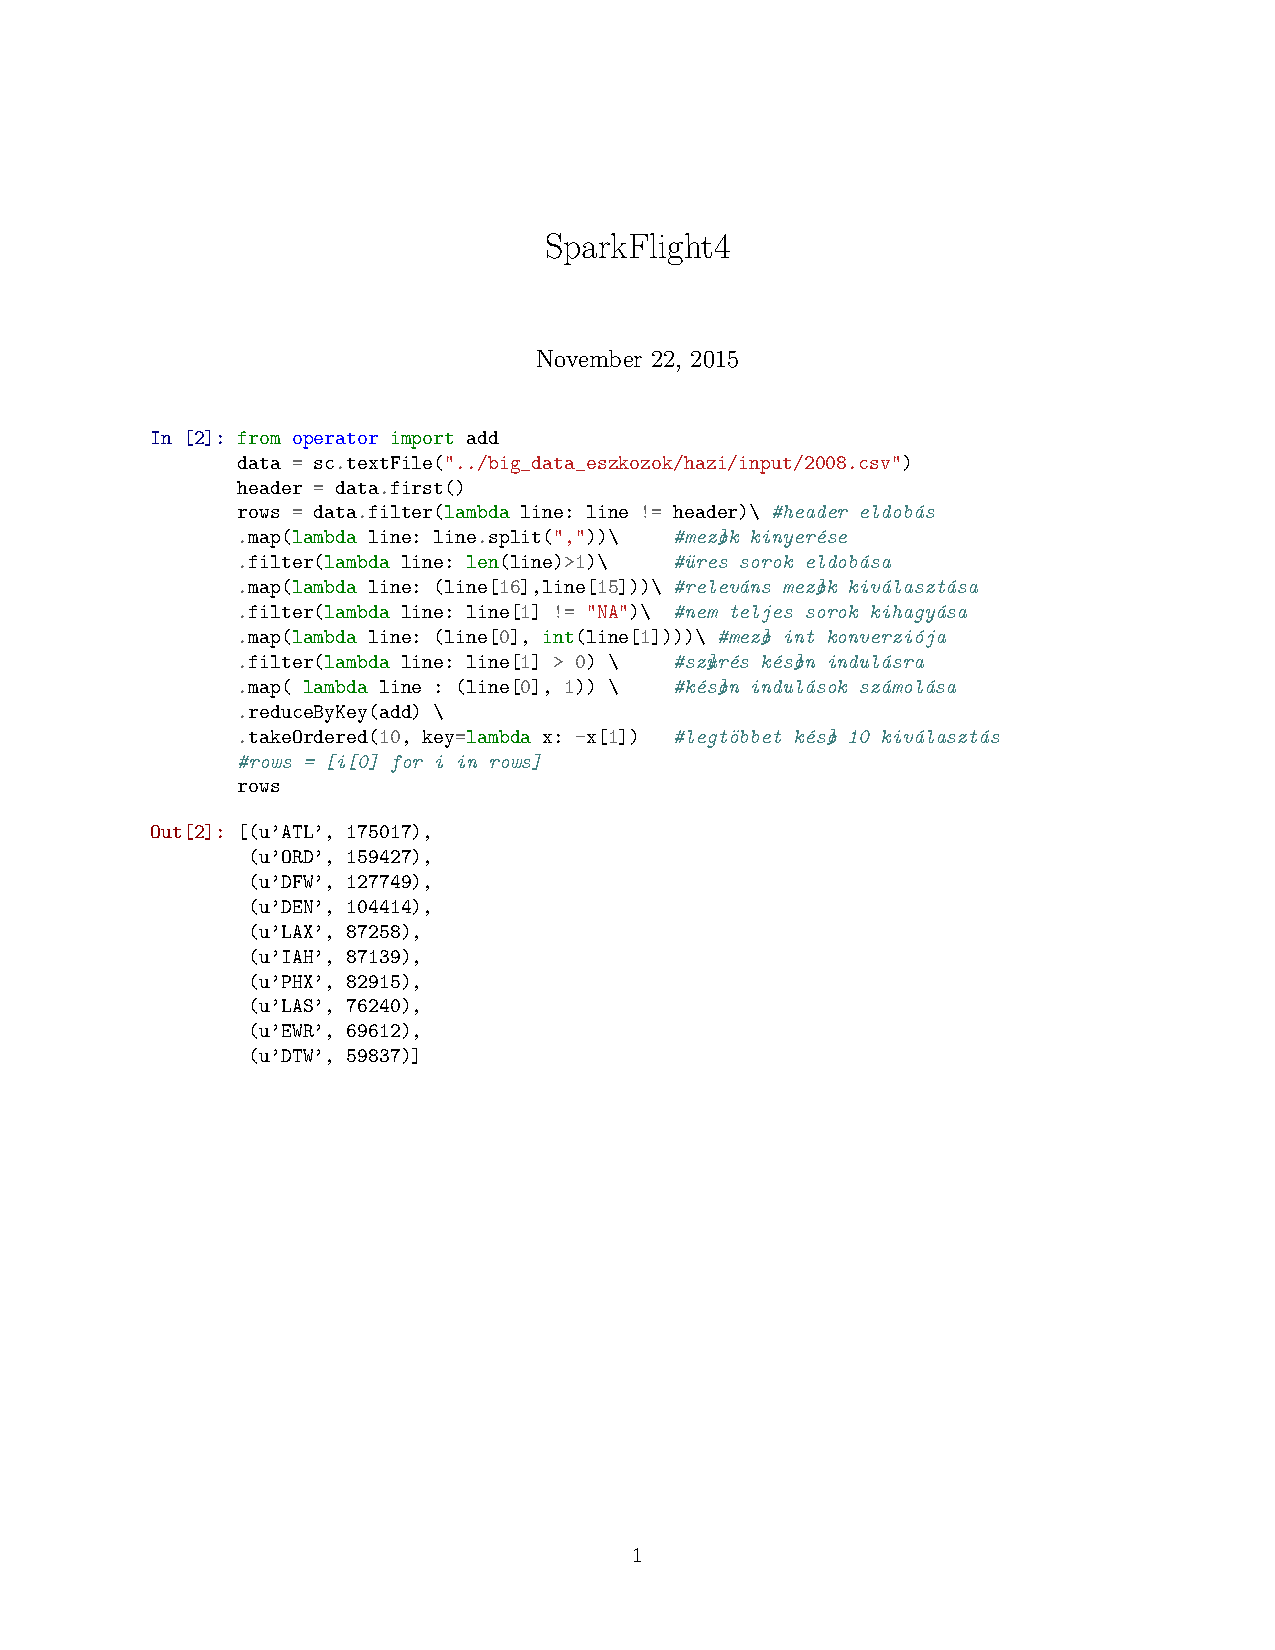
\includegraphics[scale=0.7,clip,trim=5mm 5mm 10mm 7cm]{figures/SparkFlight4.pdf}
\end{frame}

%------------------------------------------------

\begin{frame}
\frametitle{Spark megjegyzések}
\begin{itemize}
\item Első próba SparkR-ben,  jobb a Python 
\includegraphics[scale=0.025]{figures/wink}
\item Spark csak python2-vel megy egyelőre, így a Jupyter-nek(Notebook) szüksége van a python2-es kernelre(ha alapból nem azzal jön, linux disztró függő)
\end{itemize}
\end{frame}

%------------------------------------------------
\section{Flight2 - Pig} % Sections can be created in order to organize your presentation into discrete blocks, all sections and subsections are automatically printed in the table of contents as an overview of the talk
%------------------------------------------------

%------------------------------------------------
\begin{frame}
\frametitle{Pig lépések}
Honnan szállt fel a legtöbb repülő?
\begin{itemize}
	\item Nem teljes adatok szűrése
		\lstinline[basicstyle=\ttfamily\color{black}]|completeRecords = FILTER flights BY ( Origin != 'NA');|
	\item Repterek listájának előállítása
		\lstinline[basicstyle=\ttfamily\color{black}]|origin = group completeRecords by Origin;|
	\item Felszállások számolása repterenként\\
		\lstinline[basicstyle=\ttfamily\color{black}]|airportLiftoffs = |
		\lstinline[basicstyle=\ttfamily\color{black}]|foreach origin generate COUNT(completeRecords), group;|
	\item Rendezés felszállások száma szerint\\
		\lstinline[basicstyle=\ttfamily\color{black}]|ordered = ORDER airportLiftoffs BY \$0 DESC;|
	\item Legnagyobb kiválasztása\\
		\lstinline[basicstyle=\ttfamily\color{black}]|limited = LIMIT ordered 1;|\\
		\lstinline[basicstyle=\ttfamily\color{black}]|projected = FOREACH limited GENERATE \$1;|
\end{itemize}
\end{frame}

%------------------------------------------------

\begin{frame}
\frametitle{Pig futtatás}
\lstinline[basicstyle=\ttfamily\color{black}]|pig -param inputCSV="input/2008.csv"|
\lstinline[basicstyle=\ttfamily\color{black}]| -param output="pigResult" -x local Flight2.pig|
\end{frame}

%------------------------------------------------

%------------------------------------------------

\begin{frame}[plain]
\Huge{\centerline{Köszönöm a figyelmet!}}
\end{frame}


%------------------------------------------------
\end{document} 
